%\info{Andrew, Simone}

In this section, we study the sensitivity of the groomed mass to variations in the value of $\alpha_s$. We begin with a discussion based on the analytic formulae. We then discuss the issue of normalized vs. unnormalized distributions. Finally, we perform a Monte Carlo study, highlighting the interplay between the sensitivity of different parts of the distribution to variations in the value of $\alpha_s$ and non-perturbative effects.


%%%%%%%%%%%%%%%%%%%%%%%%%%%
\subsection{Analytic Understanding}\label{sec:analytic}
%%%%%%%%%%%%%%%%%%%%%%%%%%%

To get an understanding of the sensitivity of the groomed mass distribution to both the value of $\alpha_s$, as well as the quark and gluon composition, it is enlightening to study the LL distribution. Here, for simplicity, we consider only the leading logs in the observable, in the resummation region. Complete expressions, can be found in \cite{Larkoski:2014wba,Frye:2016aiz,Marzani:2017kqd,Marzani:2017mva}. The LL result at fixed coupling for the cumulant distribution for $\beta=0$ in the resummation region takes the form
\begin{align}
\Sigma(\ecf{2}{2})=\exp\left[ - \frac{\alpha_s C_i}{\pi} \log(\zcut) \log (\ecf{2}{2}) \right]\,.
\end{align}
This highlights that for $\beta=0$, the groomed jet mass is a single logarithmic observable, and therefore does not exhibit the standard Sudakov behavior.
Differentiating, we obtain the spectrum
\begin{align}
\ecf{2}{2}  \frac{d\sigma}{d \ecf{2}{2}}=   - \frac{\alpha_s C_i}{\pi} \log(\zcut)   \exp\left[ - \frac{\alpha_s C_i}{\pi}  \log(\zcut) \log (\ecf{2}{2}) \right]
\end{align}
Here we immediately see several interesting consequences. In the resummation region, the slope by the product $\alpha_s C_i$, where $C_i$ is the Casimir, namely $C_A$ for gluons, and $C_F$ for quarks. We therefore see that the groomed mass is indeed sensitive to the value of $\alpha_s$. Due to the larger color charge of gluons, we expect that samples of pure gluon jets would have a significantly higher sensitivity to the value of $\alpha_s$.  We will see that this expectation is indeed born out in our Monte Carlo simulations.  

%Should try to get to the point where we can say something about where the sensitivity in the distribution comes from (e.g. slope in log scale is proportional to $C_F\times \alpha_s$).  At the very least, it would be good to write down the LL (or even NLL) functional form for the angularities that we used (it is in the code we got from Ian (LL) and Gregory (NLL)).  Could also punt this to Sec.~\ref{sec:templates} where we will show the templates (could then just give a ref).
%
%\begin{comment}
%The Soft Drop grooming procedure~\cite{Larkoski:2014wba} takes a jet
%with momentum $p_t$ and radius $R$. It re-clusters its constituents
%using the Cambridge/Aachen (C/A) algorithm \cite{Dokshitzer:1997in,
%  Wobisch:1998wt} and iteratively performs the following steps:
%\begin{enumerate}
% \item it de-clusters the jet into 2 subjets $j \to j_1 + j_2$;
% \item it checks the condition 
%\begin{equation}\label{eq:sd-condition}
%\frac{\min (p_{t1} , p_{t2})}{p_{t1}+p_{t2}} > \zcut \left(
%  \frac{\theta_{12}}{R}\right)^\beta\,;
%\end{equation}
%\item if the jet passes the condition, the recursion stops; if not the
%  softer subjet is removed and the algorithms goes back to step 1 with
%  the hardest of the two subjets. 
% \end{enumerate}
%In the case $\beta=0$ Soft Drop essentially reduces to mMDT~\cite{Dasgupta:2013ihk},
% albeit without any actual mass-drop condition. Moreover, while the
% original MDT~\cite{Butterworth:2008iy} algorithm imposed a cut on the ratio of angular distances
% to masses, a so-called $\ycut$, the mMDT variant instead cuts on
% momentum fractions~\cite{Dasgupta:2013ihk} (see
% e.g. \cite{Dasgupta:2013ihk,Dasgupta:2016ktv} for a comparison
% between $\ycut$ and $\zcut$).
% \end{comment}
%
%Notes (order not meaningful): Plot of the two calculations for softdrop mass?  Show plots of the ATLAS and CMS measurements?  Actually, I'm not sure we can show CMS since it is only preliminary.  Say something about mass versus $k_t$?
%







%%%%%%%%%%%%%%%%%%%%%%%%%%%
\subsection{Parton Shower Monte Carlo Study}
%%%%%%%%%%%%%%%%%%%%%%%%%%%

From the point of view of fitting for $\alpha_s$, a good observable is one whose probability distribution changes significantly with variations in $\alpha_s$.  However, many observables that significantly change with $\alpha_s$ are also very sensitive to non-perturbative effects, such as the multiplicity inside jets.  In this section, many angularities are studied to quantify the tradeoff between the sensitivity to $\alpha_s$ and the robustness to non-perturbative effects.  Given two probability distributions $f$ and $g$, define the separation power $\Delta(f,g)$~\cite{Harrison:1998yr} as

\begin{align}
\label{eq:seppower}
\Delta(f,g)=\frac{1}{2}\int d\lambda \frac{(f(\lambda)-g(\lambda)^2}{f(\lambda)+g(\lambda)}.
\end{align}

\noindent As defined by Eq.~\ref{eq:seppower}, the separation power is a number in $[0,1]$ where $\Delta=1$ if and only if $f=g$ a.e.  If $f$ is the nominal probability distribution of some observable and $g$ the distribution of the same observable with a different value of $\alpha_s$, we would like $\Delta(f,g)$ close to 1 (sensitivity).  In contrast, if $g$ is the same as $f$ with some variation in the non-perturbative effects, then we would like $\Delta(f,g)$ to be close to $0$ (robustness).  The plane used to study the tradeoff between sensitivity and robustness is shown in Fig.~\ref{fig:robustnessschematic}.  Not all information about $\alpha_s$ sensitivity is captured by a single point in Fig.~\ref{fig:robustnessschematic} because sensitivity to non-perturbative effects could be in regions of low $\alpha_s$ sensitivity and vice versa.  Therefore, it is also useful to study the integrand of Eq.~\ref{eq:seppower} as a function of the angularity $\lambda$.

\begin{figure}[h!]
\begin{center}
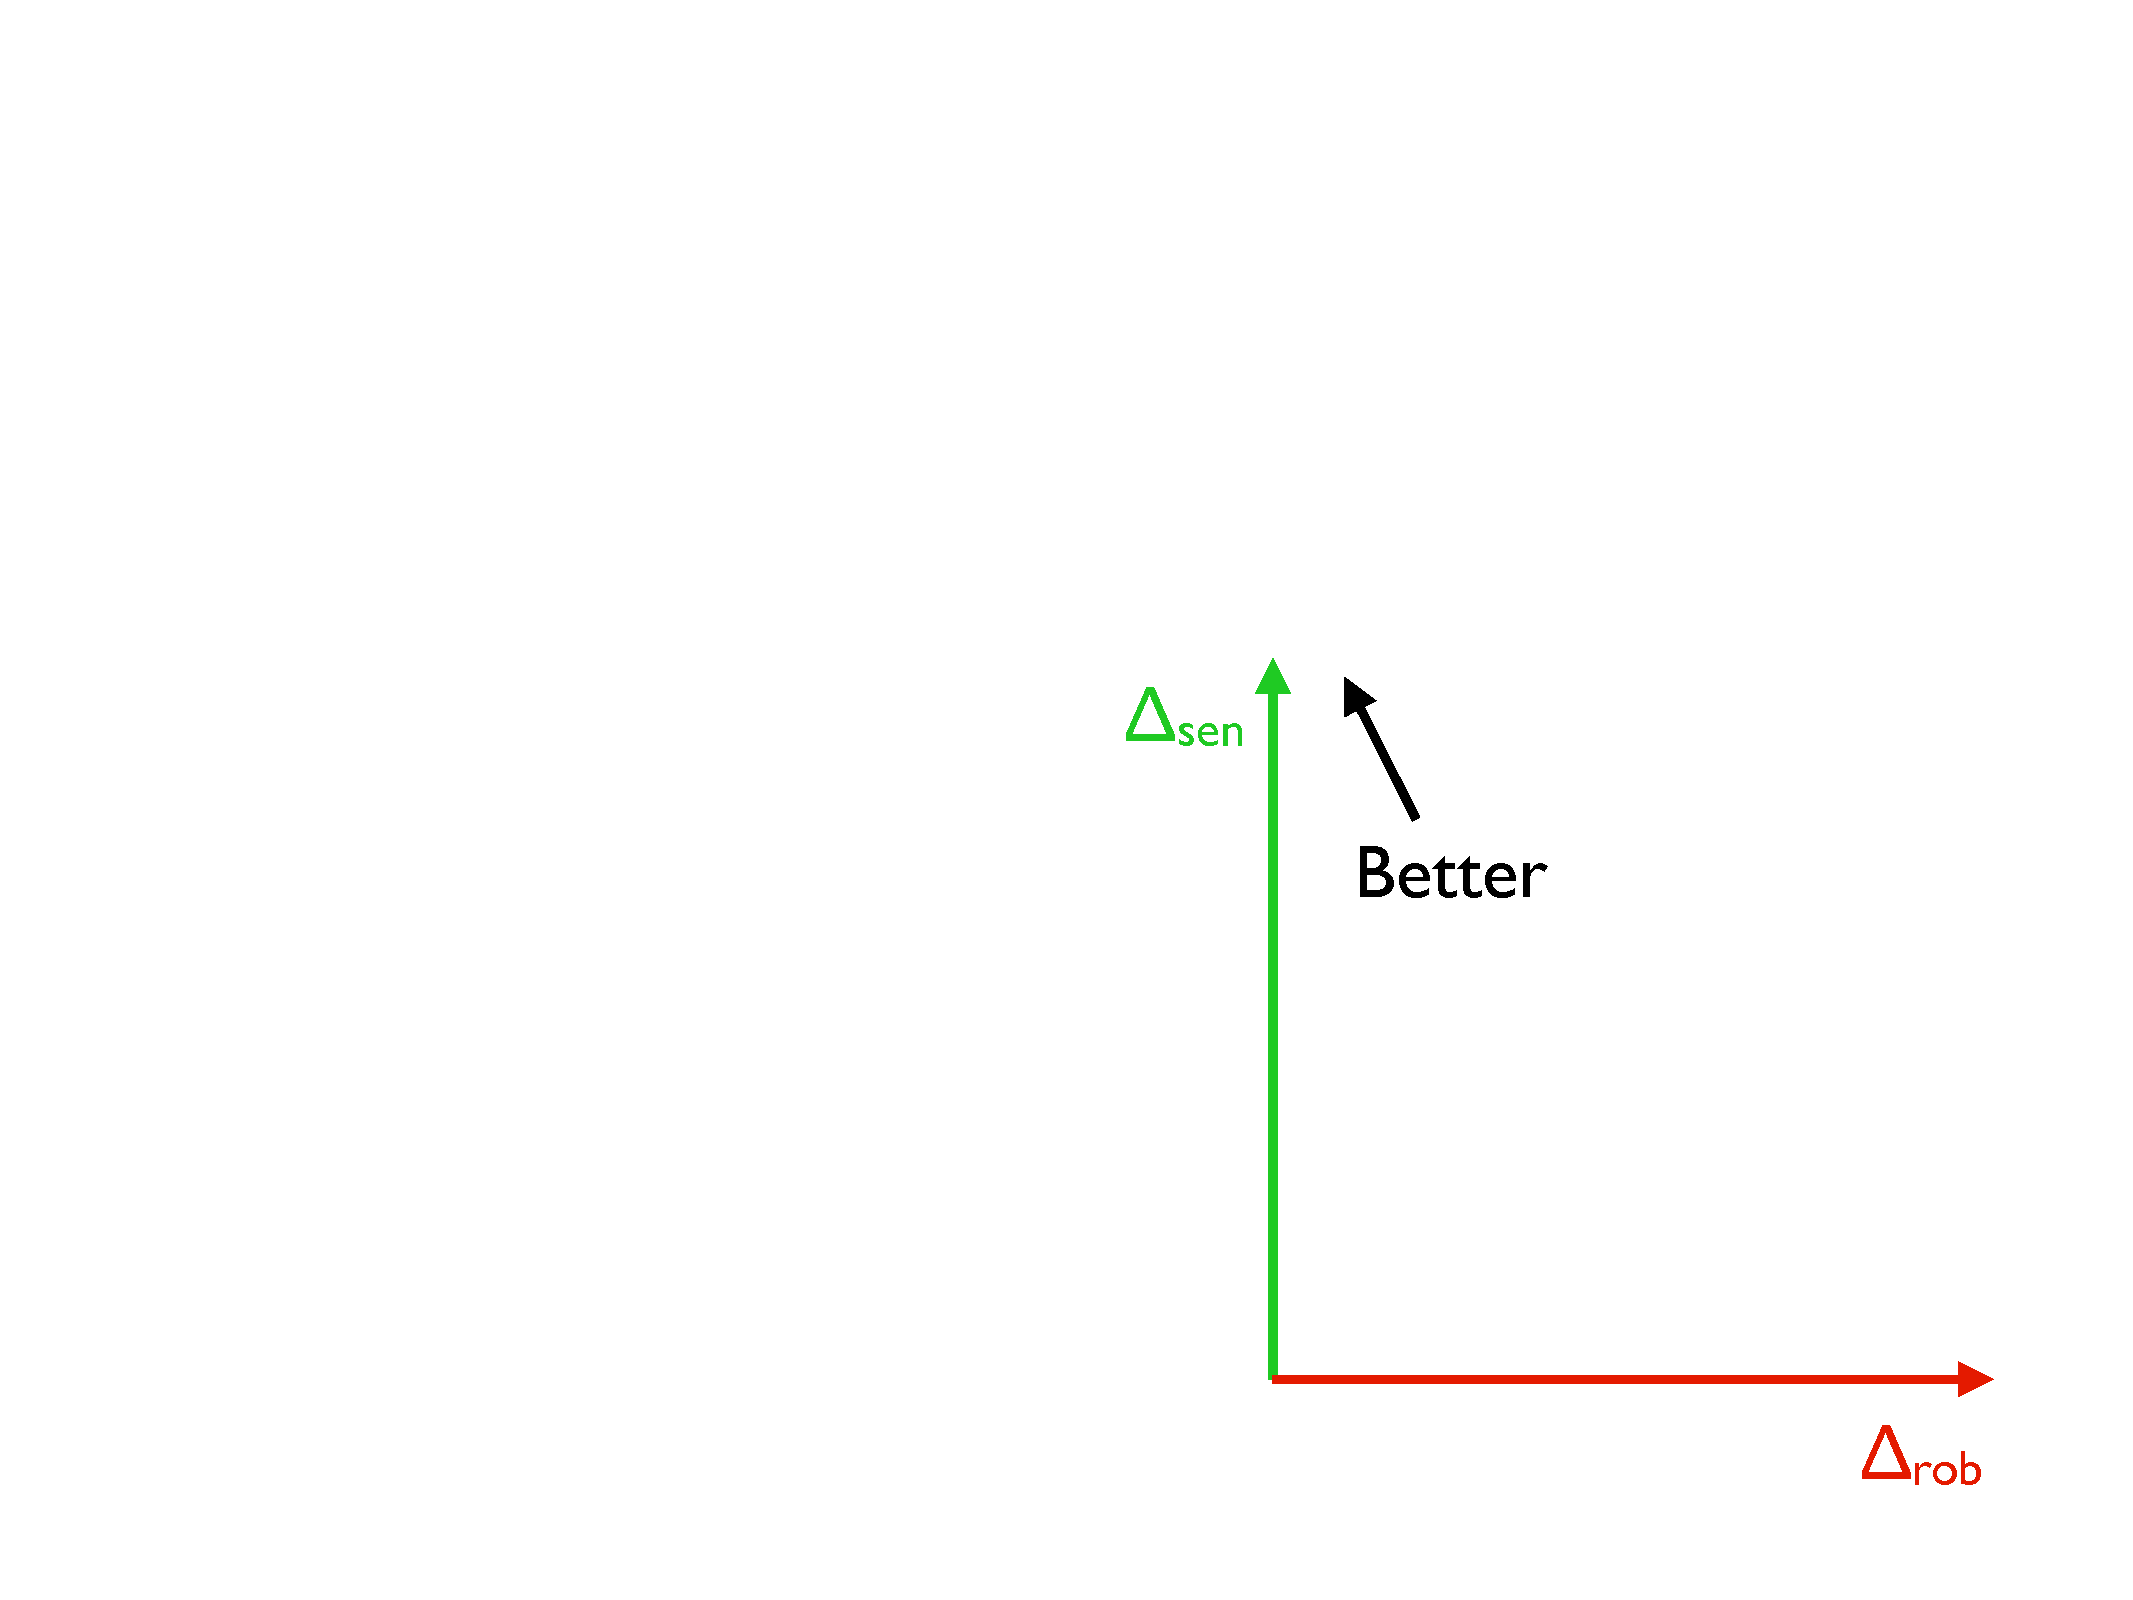
\includegraphics[width = 0.4\columnwidth]{figures/robustnessschematic.pdf}
\end{center}
\caption{A schematic diagram to illustrate the sensitivity-robustness plane defined by the separation power defined in Eq.~\ref{eq:seppower}.}
\label{fig:robustnessschematic}
\end{figure}

The sensitivity-robustness tradeoff is studied using (formally) leading logarithm PS MC programs Herwig 7.1~\cite{Bellm:2015jjp,Reichelt:2017hts} with the default tune and Pythia 8.223~\cite{Sjostrand:2006za,Sjostrand:2014zea} with the tune 4C.  Results are presented for separately for quark and gluon jets, simulated with $Z+q$ and $Z+g$.  A variety of angularities (as defined in Sec.~\ref{sec:shape_def}), with $\alpha\in\{0.5,1.0, 2.0\}$ corresponding to the Les Houches Angularity~\cite{Gras:2017jty}, width, and mass, respectively.  Additionally, various grooming parameters are studied by varying $\beta\in\{0,1,2\}$ and $z_\text{cut}\in \{0.05,0.1,0.2\}$.  

\begin{figure}[h!]
\begin{center}
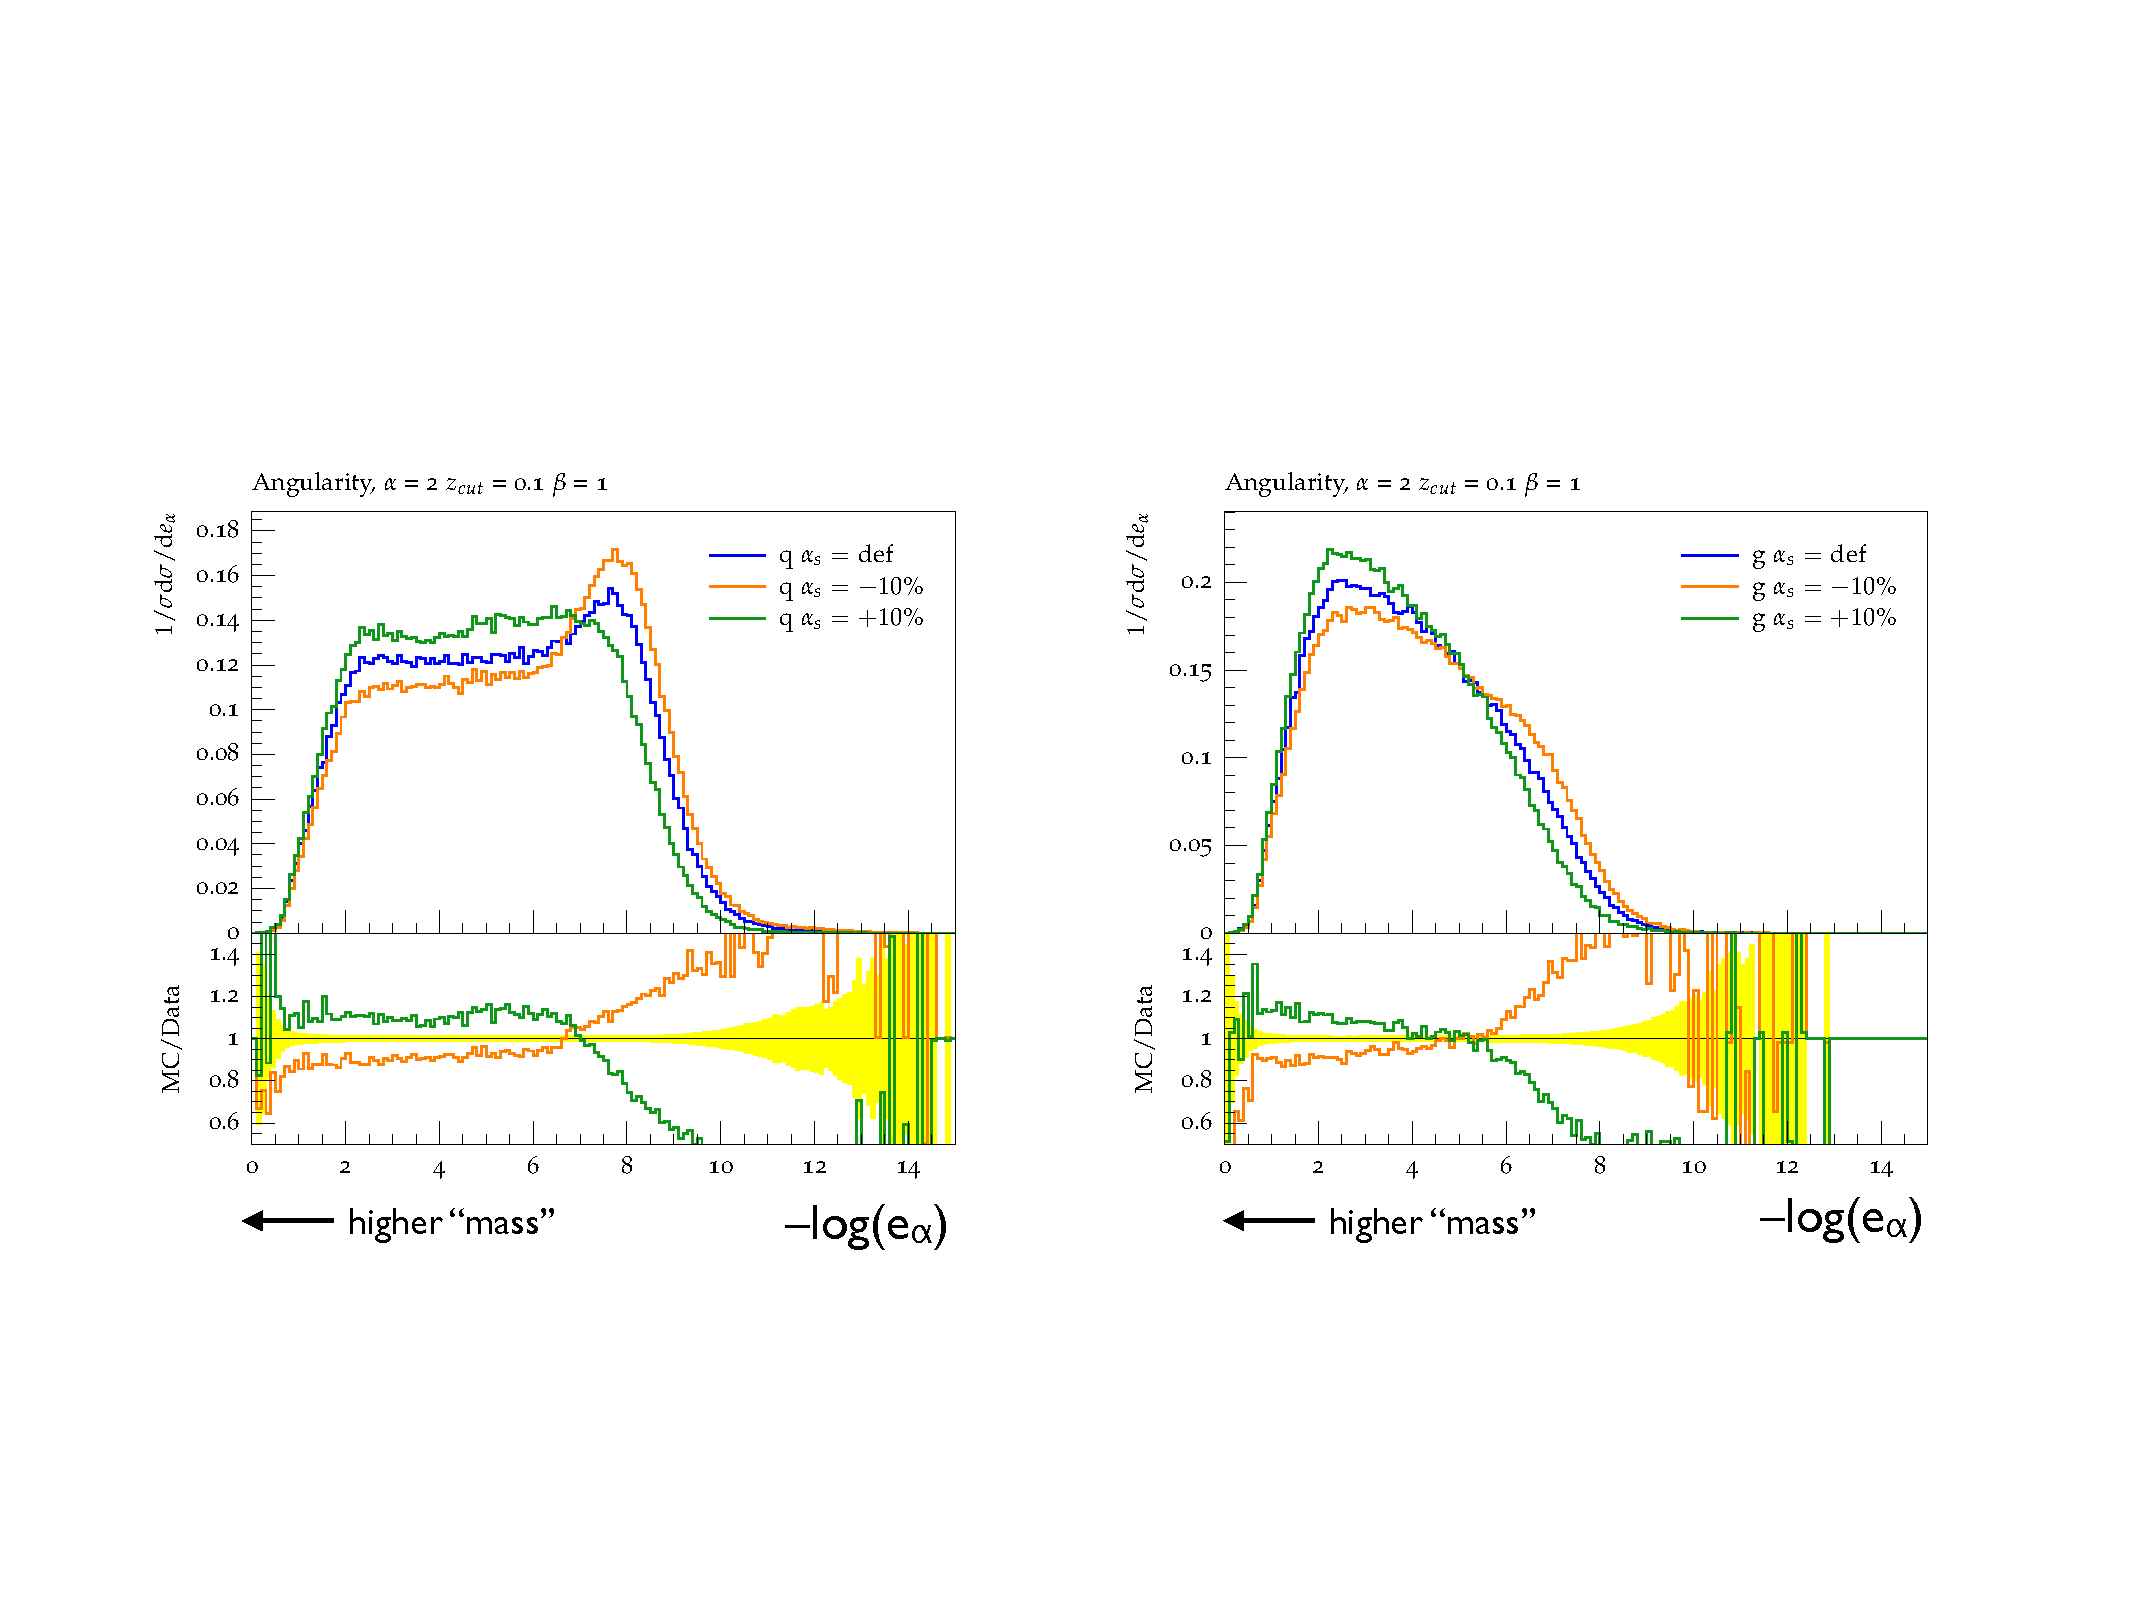
\includegraphics[width = 0.99\columnwidth]{figures/sensitivity.pdf}
\end{center}
\caption{The distribution of the normalized squared jet mass ($e_2$) for quark jets (left) and gluon jets (right).  Higher values of the mass are on the left.  The blue line uses $\alpha_s=0.118$ while the green and orange lines have the value of $\alpha_s$ varied by $10\%$.  The lower panels show the ratio with respect to the $\alpha_s=0.118$ curve.\textbf{Maybe cut the x-axis at high values?  Maybe comment what the picture looks like for Pythia?}}
\label{fig:sensitivity}
\end{figure}

\begin{figure}[h!]
\begin{center}
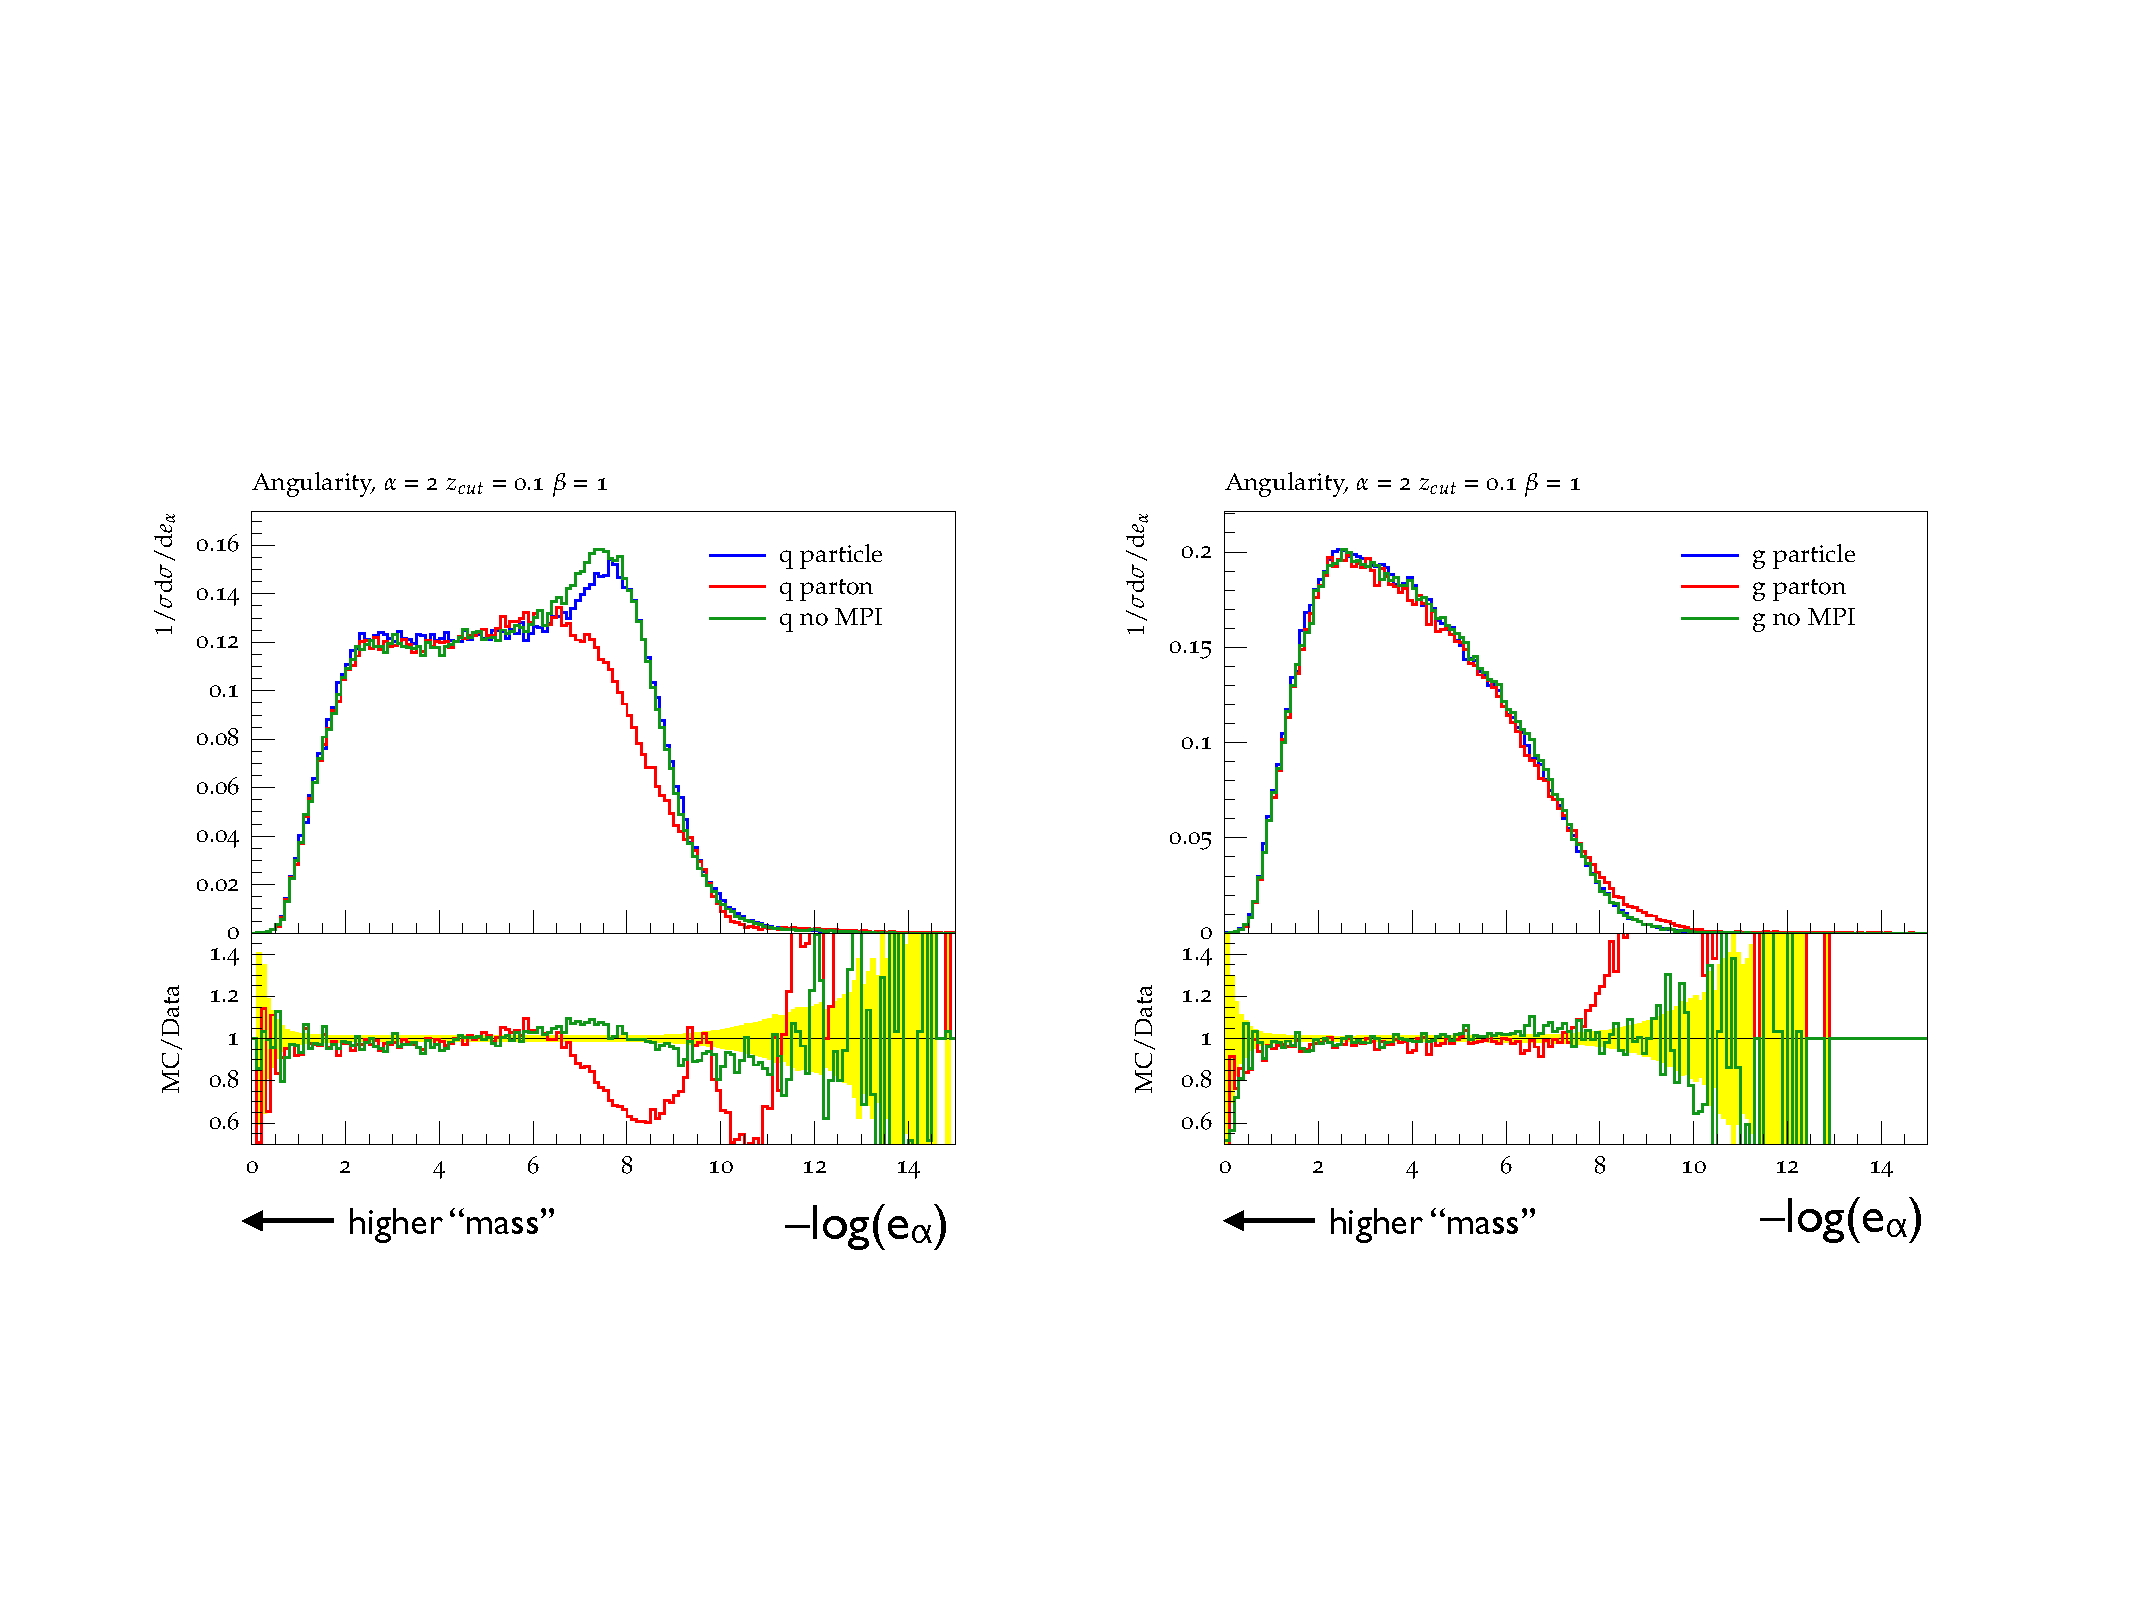
\includegraphics[width = 0.99\columnwidth]{figures/robustness.pdf}
\end{center}
\caption{The distribution of the normalized squared jet mass ($e_2$) for quark jets (left) and gluon jets (right).  Higher values of the mass are on the left.  The blue line shows the default particle-level simulation that includes the standard cluster hadronization model.  The red curve has hadronization turned off and the green curve has hadronization, but with the Herwig model for multiple parton interactions (MPI) turned off. \textbf{Maybe cut the x-axis at high values?  Maybe comment what the picture looks like for Pythia?}}
\label{fig:robustness}
\end{figure}

\begin{figure}[h!]
\begin{center}
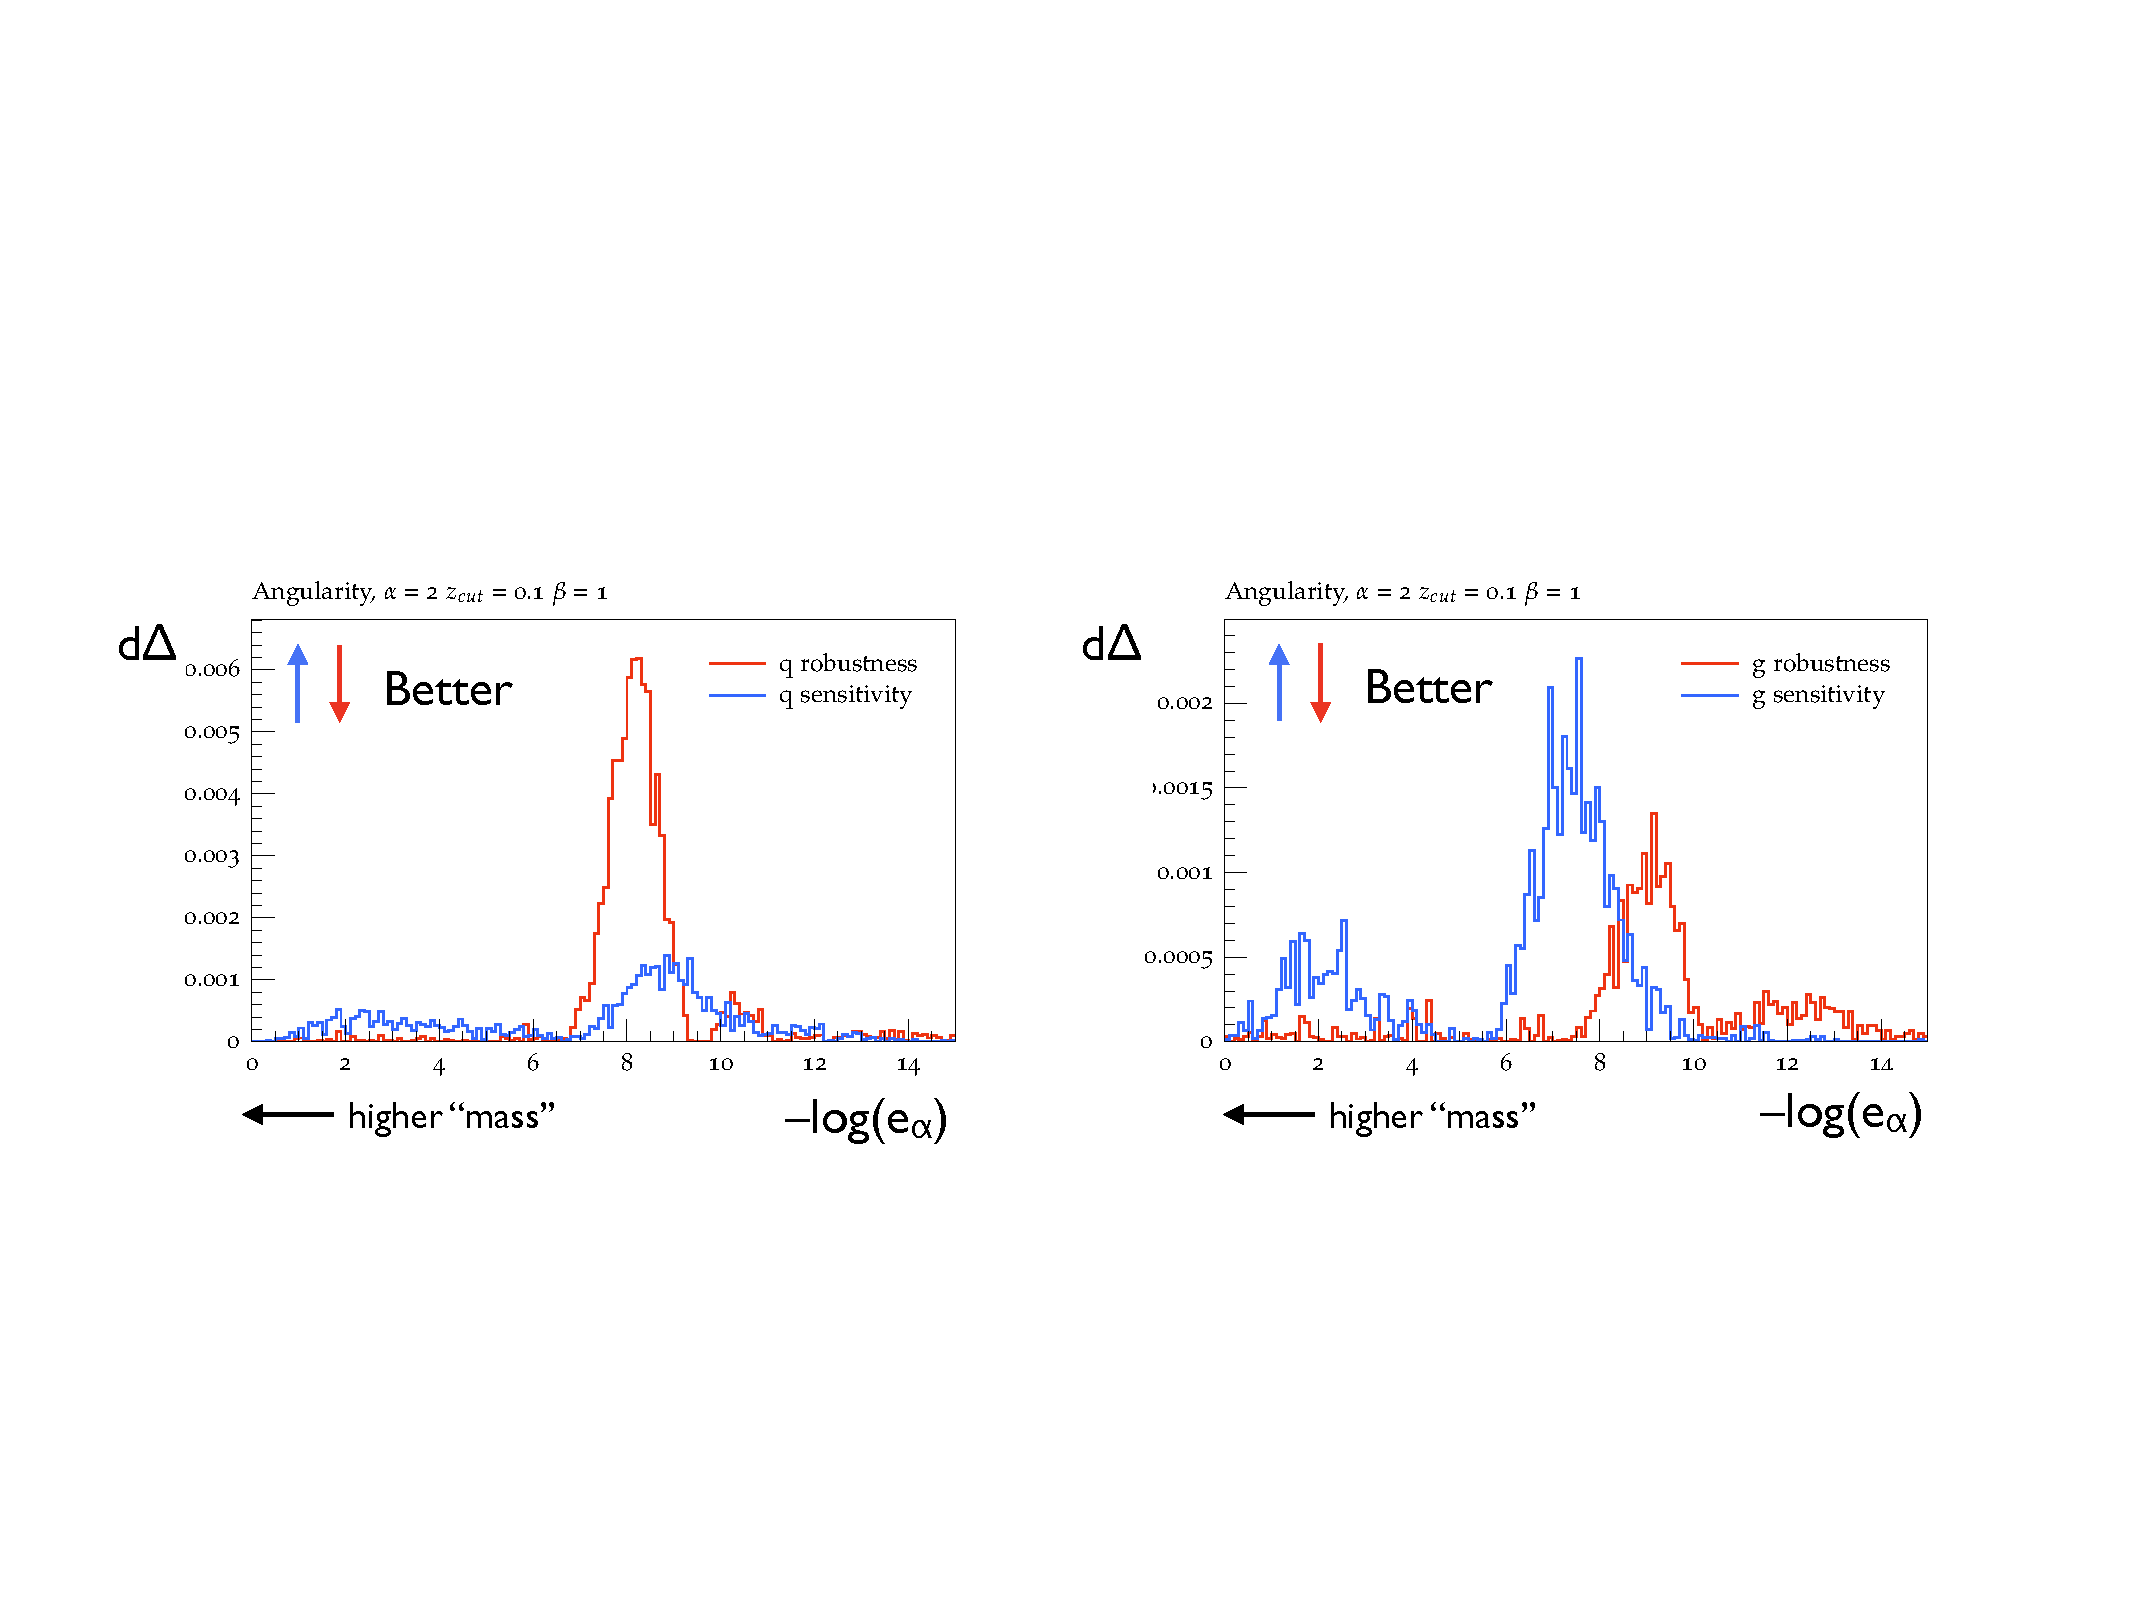
\includegraphics[width = 0.99\columnwidth]{figures/differentialseparation.pdf}
\end{center}
\caption{The integrand of Eq.~\ref{eq:seppower} for the normalized squared jet mass ($e_2$) for quark jets (left) and gluon jets (right).  Higher values of the mass are on the left.  In $f$ from Eq.~\ref{eq:seppower} is the same for red and blue, but for blue (robustness), $\alpha_s$ is varied by 10\% and for red (robustness), hadronization is turned off.}
\label{fig:differentialseparation}
\end{figure}

Figures~\ref{fig:sensitivity} and~\ref{fig:robustness} show the distribution of the normalized squared jet mass ($e_2$) for quark and gluon jets.  To the left of the low-mass peak, the shape of the $e_2$ distribution is nearly flat for quarks and nearly linear (in the log-space) for gluons.  Increasing $\alpha_s$ shifts the quark distribution up but has nearly no impact on the shape of the distribution below the peak.  The size of the peak is significantly impacted by the value of $\alpha_s$.  In contrast, the slope of the distribution for gluons changes with the variations in $\alpha_s$.  Figure~\ref{fig:sensitivity} shows the same $e_2$ distribution, but now with variations in the modeling of non-perturbative effects.  The low-mass peak for quarks is entirely due to hadronization effects.  According to the Herwig 7 MC, the impact of hadronization is much smaller for gluon jets.  Figure~\ref{fig:differentialseparation} shows the distribution of the differential separation power (integrand of Eq.~\ref{eq:seppower}), using the variation with $\alpha_s$ as the sensitivity and the change from turning off hadronization as the robustness.  For quark jets, Figs.~\ref{fig:sensitivity} and~\ref{fig:robustness} showed that the biggest variations with $\alpha_s$ occurred at low mass which is also where non-perturbative effects are largest.  This corresponds to the peak in the blue and red distributions in Fig.~\ref{fig:differentialseparation} occurring in nearly the same location.  In contrast, the peaks are more well-separated in Fig.~\ref{fig:differentialseparation} for gluon jets and the blue is shifted to higher mass values where there is more perturbative control.  

\begin{figure}[h!]
\begin{center}
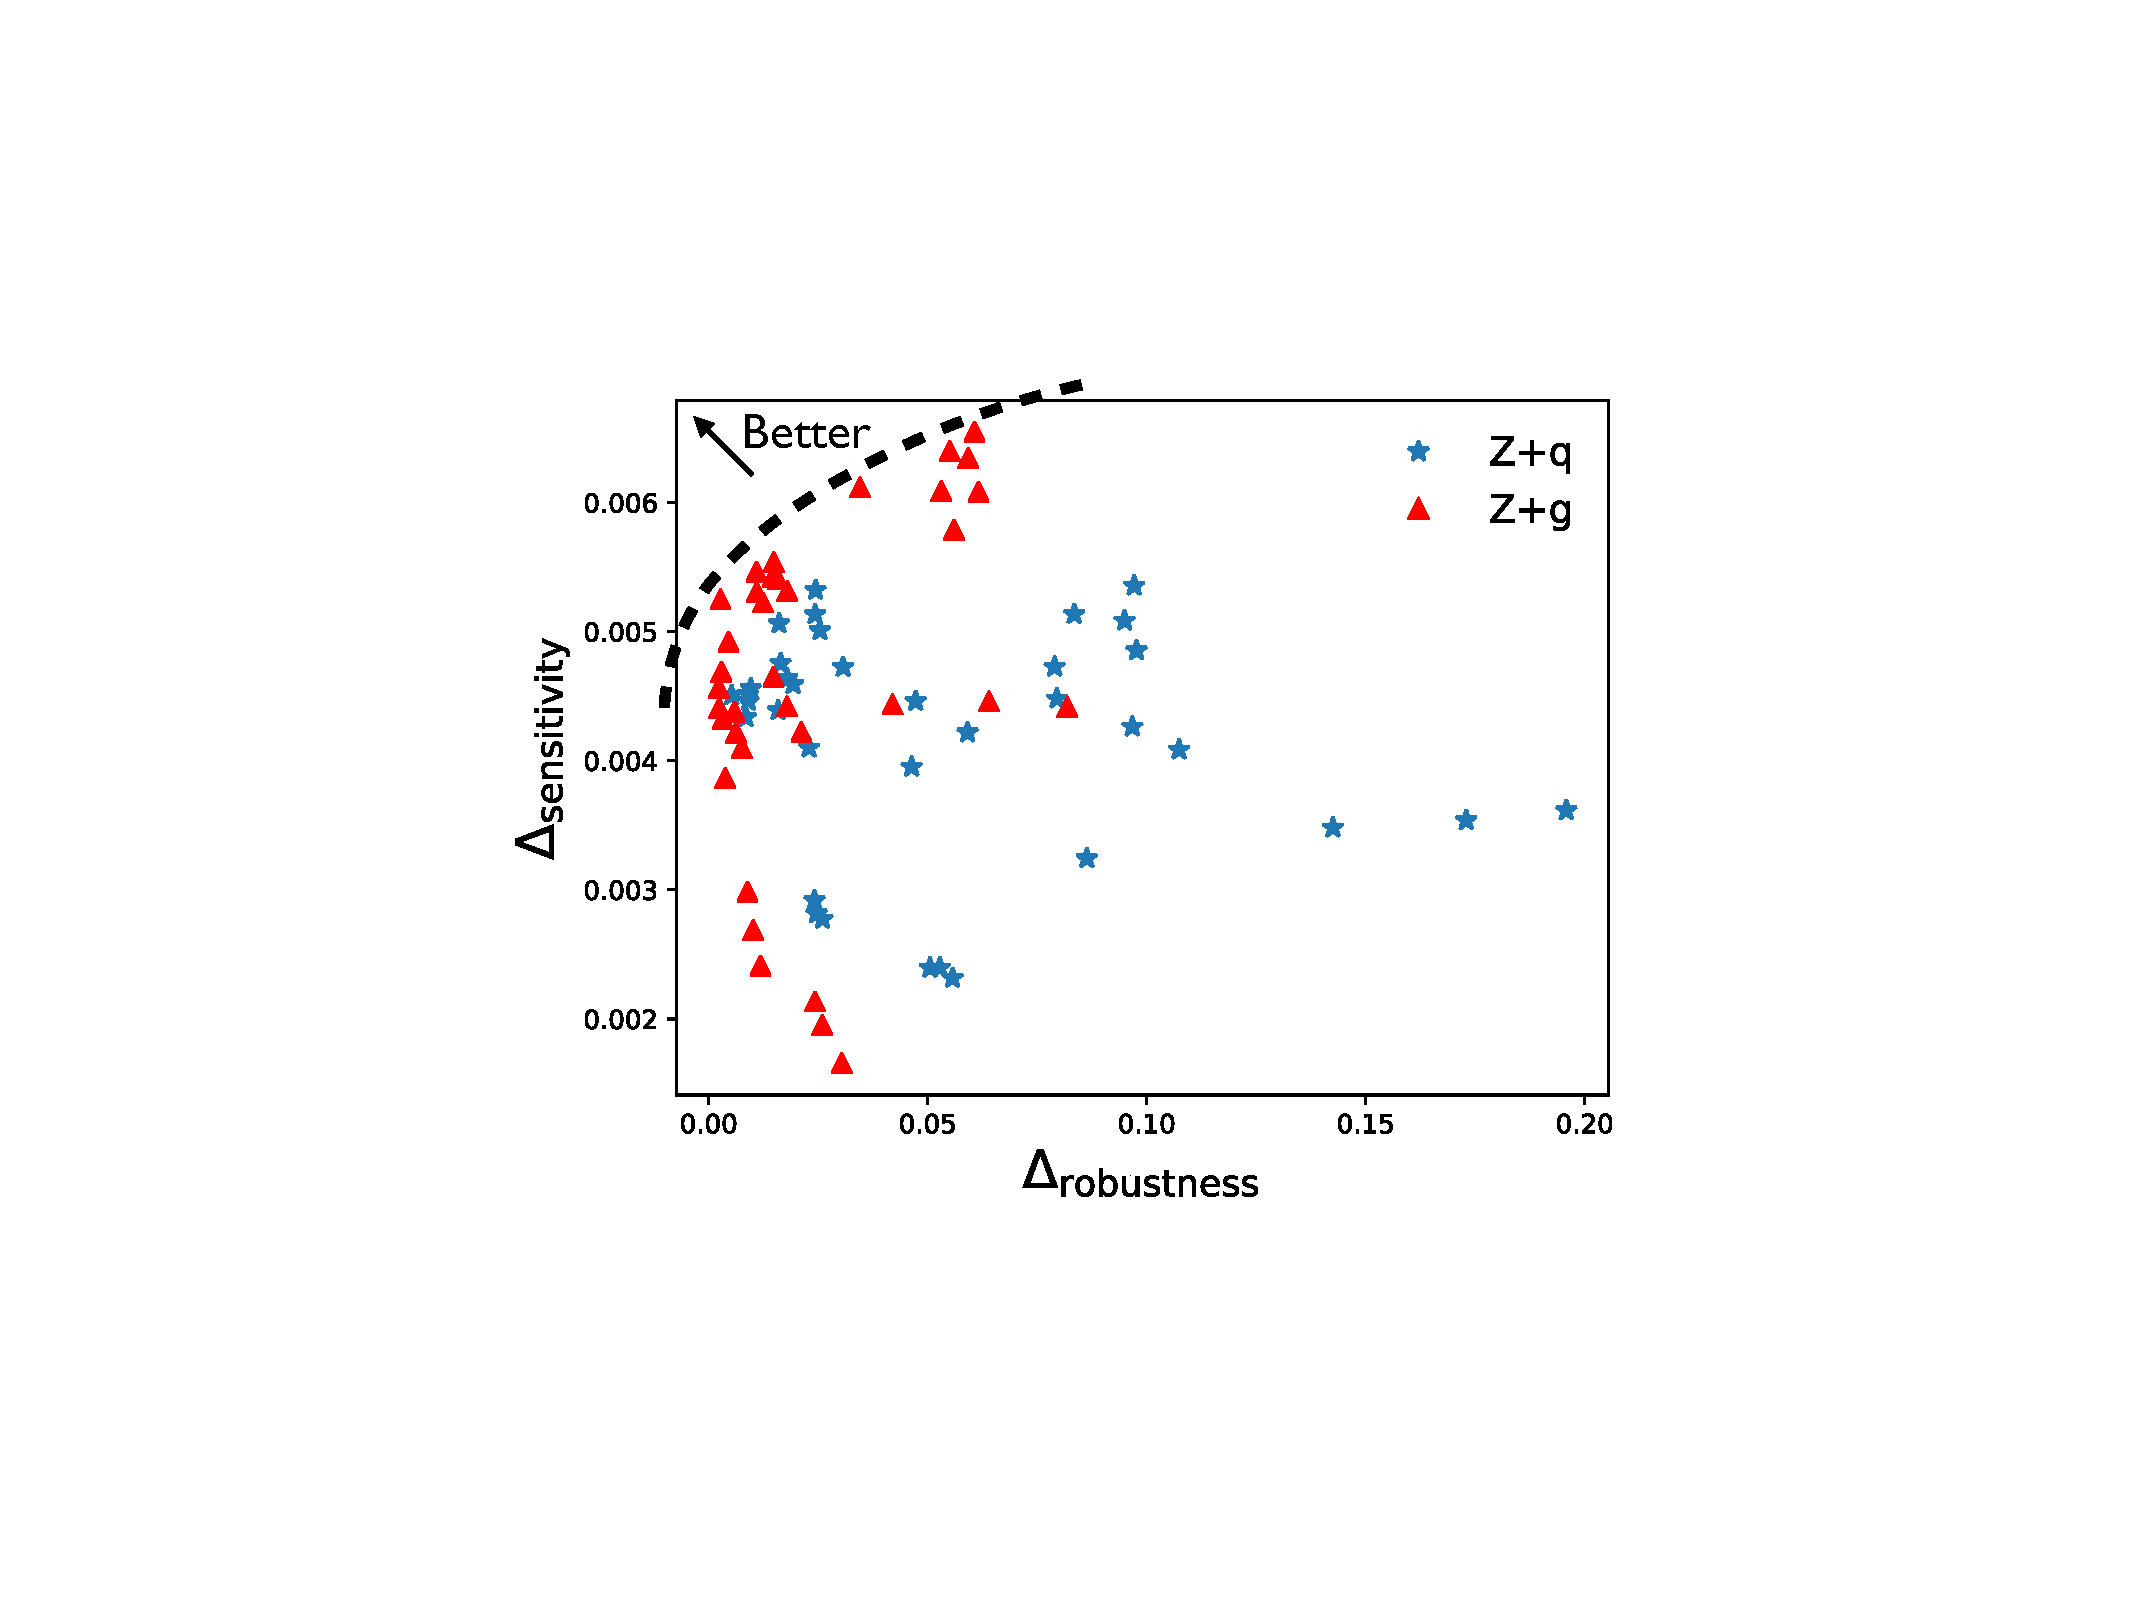
\includegraphics[width = 0.6\columnwidth]{figures/robseptradeoff.pdf}
\end{center}
\caption{The tradeoff between sensitivity and robustness for the 36 angularities studied in this section.  Stars represent quark jets and triangles represent gluon jets. \textbf{Should explain where 36 comes from (includes $\theta$).  How does this picture change if we truncate the range of $\lambda$?  (see Gregory's formula).}}
\label{fig:robseptradeoff}
\end{figure}

A summary of the sensitivity-robustness tradeoff for many angularities is presented in Fig.~\ref{fig:robseptradeoff}.  As already observed for the jet mass, gluons tend to have a superior sensitivity and robustness compared with quarks.  This is not surprising, as gluons have more perturbative radiation than quarks ($C_A>C_F$).  The jet mass has $(\Delta_\text{sensitivity},\Delta_\text{robustnes})=(?,?)$.  The angularities with the highest quark and gluon sensitivity and robustness are ?, ?, and ?.   Conclusion + transition sentence(s).









%%%%%%%%%%%%%%%%%%%%%%%%%%%
\subsection{The Issue of Casimir Scaling}
\label{sec:casimir}
%%%%%%%%%%%%%%%%%%%%%%%%%%%



While we have illustrated that the groomed jet mass observable provides a sensitivity to $\alpha_s$ particularly for gluon jets, one problem that is immediately clear from \Sec{sec:analytic} is that the leading behavior of the distributions is always dominated by the product $\alpha_s C_i$. While this is broken at higher perturbative orders, it implies that at lowest order there is a complete degeneracy of the value of $\alpha_s$ and the quark vs. gluon fraction of jets. This problem is not faced at $e^+e^-$ colliders.

There are a variety of different approaches to overcome this problem, each with their own advantages and disadvantages. First, we note that the quark and gluon fractions are perturbatively calculable given the pdfs. Therefore, perturbatively calculating the quark and gluon fractions inputs the most possible information, and should correspondingly lead to the best sensitivity for $\alpha_s$. However, it has the downside that it also introduces sensitivity to the pdfs, which in principle should be fitted along with $\alpha_s$. This difficulty also enters into other extractions at the LHC, for example the $3$-$2$ jet rate or the EEC. However, a hope using jet substructure was that the sensitivity to the pdfs could be minimized.

A second approach is to simultaneously fit for the quark (or gluon) fraction. Due to the fact that the two fractions must add to unity, this introduces a single additional parameter (see Fig.~\ref{fig:analyticbanana}). The degeneracy between the quark and gluon fraction and $\alpha_s$ is broken by higher order effects. Furthermore, different $\ecf{2}{\alpha}$ have different dependence on $\alpha_s$ and $C_i$ at higher orders. Therefore, the measurement of multiple angularities would allow the degeneracy to be broken. However, from a theoretical perspective, this significantly complicates the analysis, and we do not believe that precise predictions will be made in the near future, except for $\alpha=2$, and perhaps $\alpha=1$. In our study in \Sec{sec:ben_study} we will consider both approaches.

It would be interesting to understand other approaches to disentangling the quark and gluon fractions and $\alpha_s$, however, we expect that this will be a limiting aspect of $\alpha_s$ extractions at the LHC.


\begin{figure}[h!]
\begin{center}
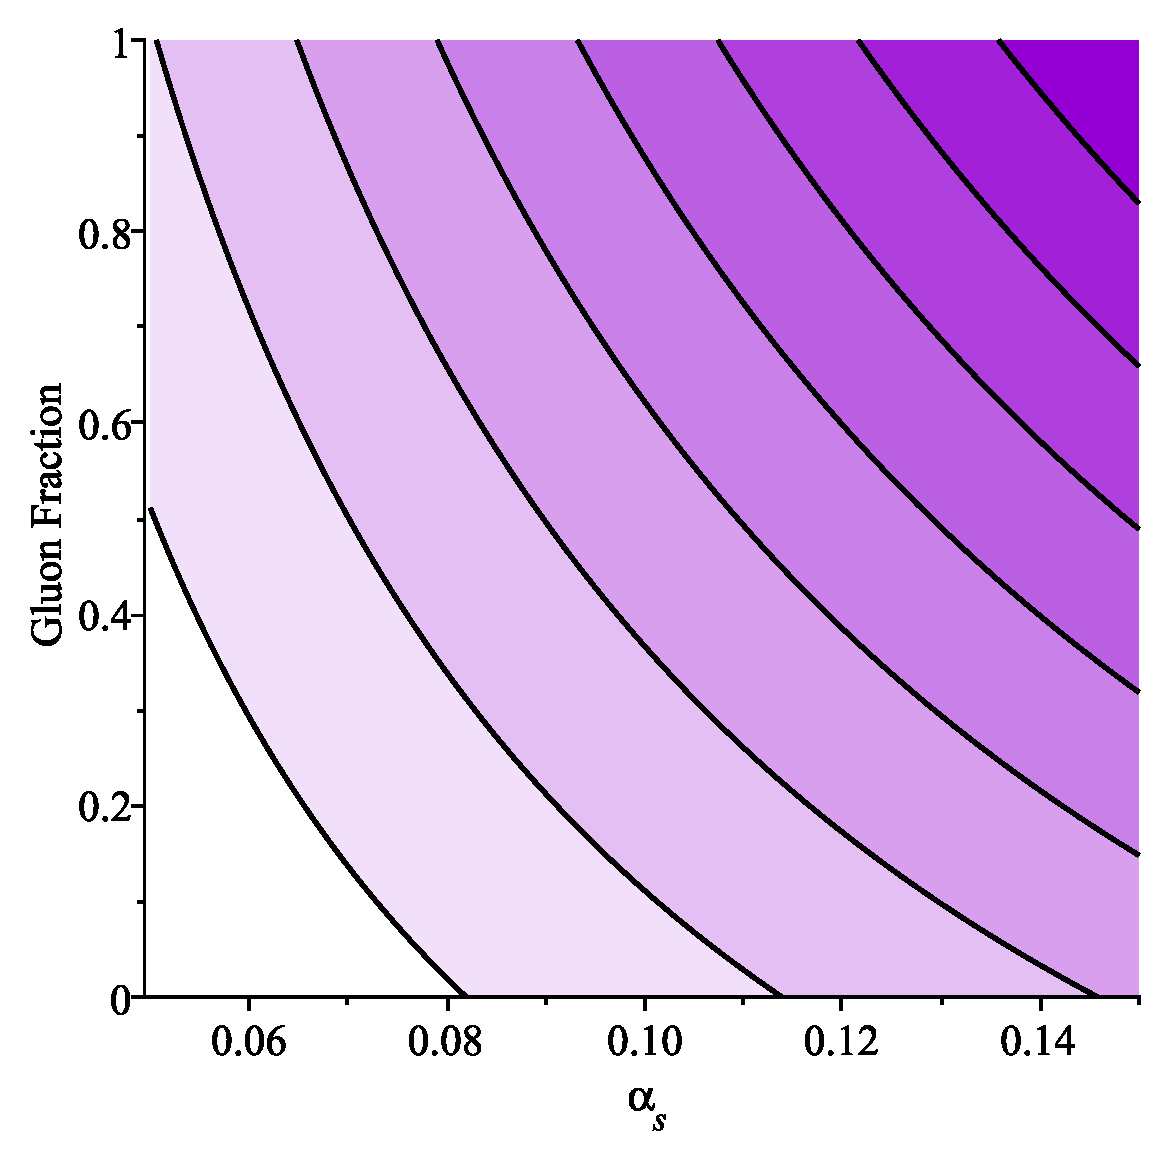
\includegraphics[width = 0.4\columnwidth]{figures/Degeneracy}
\end{center}
\caption{The slope of the probability distribution of $\ecf{2}{2}$ (as a function of $\log(\ecf{2}{2})$) is proportional to $\alpha_s(C_Af_g+C_F(1-f_g))$, which is plotted above.  The degeneracy between $\alpha_s$ and $f_g$ (gluon fraction) are represented by the banana-shaped isocontours. }
\label{fig:analyticbanana}
\end{figure}


%%%%%%%%%%%%%%%%%%%%%%%%%%%
\subsection{Normalized vs. Unnormalized Distributions}
%%%%%%%%%%%%%%%%%%%%%%%%%%%

In addition to the complication of quark and gluon fractions, another issue which appears for the extraction of $\alpha_s$ from jet substructure, as compared to $e^+e^-$ event shapes is the issue of normalization.\footnote{We thank Gavin Salam for interesting discussions regarding the issue of normalization.} Unlike in $e^+e^-$, the born dijet cross section in $pp$ is sensitive to the value of $\alpha_s$. This implies that the rate itself, in particular, the absolute quark and gluon jet rates carries information regarding $\alpha_s$. 

Here we will focus on using the normalized distribution. We do this for three reasons. First, we would like this to be a true measurement of $\alpha_s$ from the jet substructure, and not be dominated by the overall rate. Second, and more importantly, it is currently only possible to perform the experimental measurement of the groomed mass precisely for the normalized distribution.  Experimentally, the absolute rate is determined by the acceptance from kinematic requirements on the jet $p_\text{T}$.  The sophisticated in-situ jet energy scale and resolution program carried out for small-radius jets~\cite{Aad:2014bia,Aaboud:2017jcu,Khachatryan:2016kdb,CMS-DP-2016-020} has not yet reached the same level of maturity for groomed large-radius jets.  However, this is simply a matter of time and efforts have already started in this direction~\cite{ATLAS-CONF-2017-063}.  A key challenge that still remains is to fully understand the correlations in the calibrations and uncertainties between the jet energy and the jet substructure observables.  Finally, the use of normalized distributions minimizes the sensitivity to the parton distribution functions.  As discussed in Sec.~\ref{sec:pertsimplicity}, grooming renders the quark and gluon angularity distributions universal.  Therefore, the measured distribution only depends on the fraction of gluon jets $f_g$ that pass the event selection.  In contrast, the total cross-section depends on the relative proportions of all possible partonic initial states.  This introduces a source of uncertainty that is not present for the normalized cross-section.  For example, the initial state could be one of $qq$, $qg$ or $gg$.  The relative proportions can be parameterized by two numbers $f_{qg}$ and $f_{gg}$ where $f_{qg}+f_{gg}=1-f_{qq}$.   Figure~\ref{fig:pdf} shows the uncertainty in the $f_{qg}$ and $f_{gg}$ from leading order PDFs.  Fixing $f_g$, which carries all of the PDF sensitivity for the shape measurement, has little effect on the uncertainty in $f_{qg}$ and $f_{gg}$.  This results in the residual PDF sensitivity from also measuring the total cross-section in addition to the shape of the angularity distribution.





One issue with using purely the normalized jet shape is that since the mass distribution starts at $\cO(\alpha_s)$. In other words, the slope of the groomed mass distribution is $\cO(\alpha_s)$. This implies that to have an $\cO(\alpha_s^2)$ uncertainty on the slope, one should have an NNLO calculation for a jet with two constituents.  In particular, this requires $2\to 3$ matrix elements. For the case of $e^+e^-$ this level of accuracy has been achieved, where the NNLO corrections to $e^+e^-\to 3$ jets are known, and are used in the extractions of $\alpha_s$. Due to recent progress in the calculation of the relevant amplitudes, we believe this is realistic.



\begin{figure}[h!]
\begin{center}
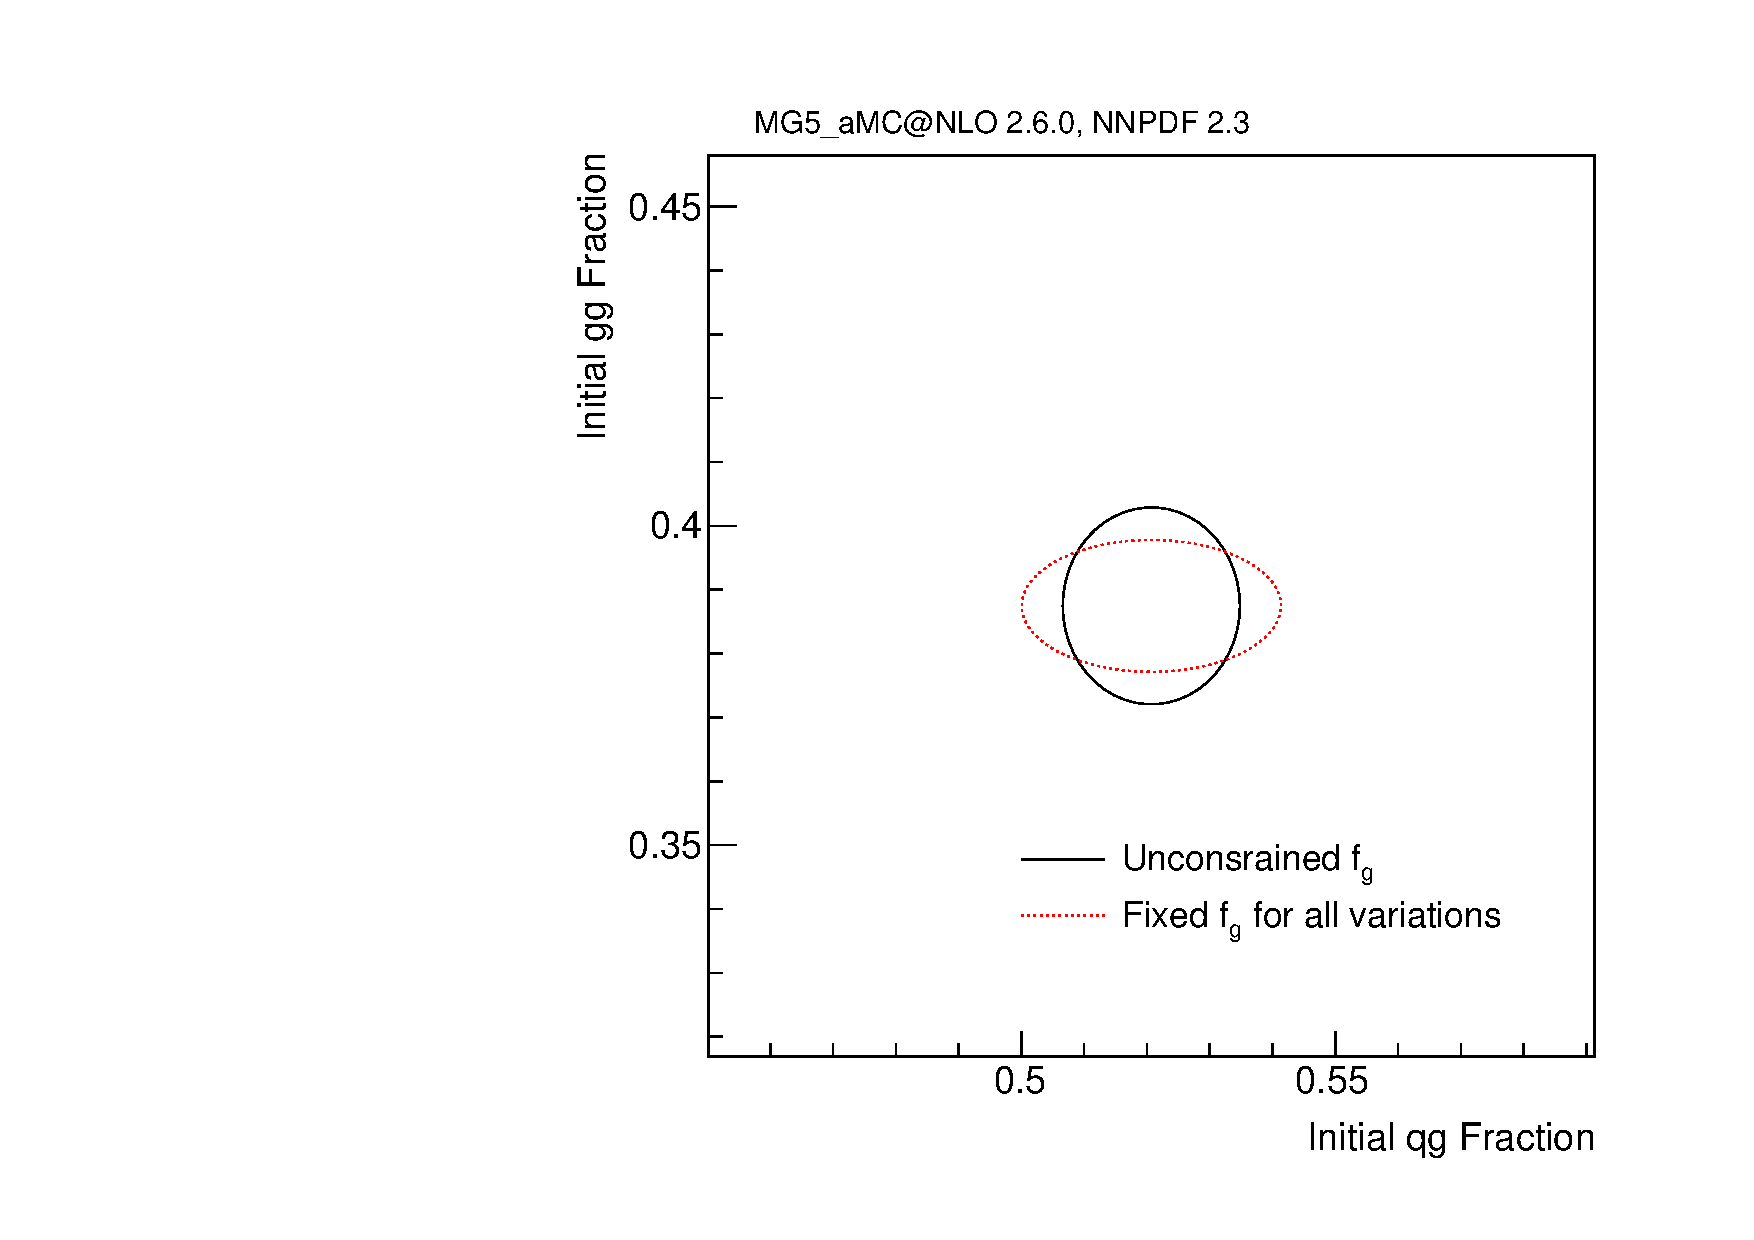
\includegraphics[width = 0.5\columnwidth]{figures/PDFs.pdf}
\end{center}
\caption{The fraction of $qg$ and $gg$ initial states for leading order dijet production simulated with MG5\_aMC 2.6.0~\cite{Alwall:2014hca} using the NNPDF 2.3~\cite{Ball:2012cx} parton distribution function (PDF) set.  The ellipses correspond to the uncertainty from the 100 error PDF sets.  For the red dashed line, the fraction of out-going gluon jets $f_g$ is constrained to be the same for all variations (and equal to the nominal PDF set).}
\label{fig:pdf}
\end{figure}





























%%%%%%
